\chapter{Machine Learning}
Machine learning algorithms can extract patterns and learn from data \cite{IanGoodfellow2016}. A brief definition of learning can be given as \cite{mitchell1997machine}
\begin{displayquote}[][]
    "A computer program is said to learn from experience \textit{E} with respect to some class of tasks \textit{T} and performance measure \textit{P}, if its performance at tasks in \textit{T}, as measured by \textit{P}, improves with experience \textit{E}."
\end{displayquote}

A task is the main objective of using an ML algorithm. For example, in an autonomous vehicle, driving the car is the task. A task is not the process of learning. Learning is used as a means to achieve an ability to accomplish a task \cite{IanGoodfellow2016}. With developments in ML methods, they have been applied to different tasks, some examples of tasks are classification, regression, transcription, machine translation, denoising \cite{IanGoodfellow2016}.

The performance measure is used to quantify how successfully a task is accomplished, equivalently, number of erroneous outputs could be used as a way of indicating a method's performance. 

Based on the above-stated definition, the ML algorithm undergoes an experience in the process of learning. This experience is generally classified into \textbf{unsupervised}, \textbf{supervised} and \textbf{reinforcement} learning.

Unsupervised learning finds the properties of the overall structure of the dataset. Clustering as an example of unsupervised learning, finds clusters within a dataset and assigns each data-point to one of them.\\In supervised learning, on the other hand, data-points that the learning algorithm experiences have a label. This label acts as a guide for the ML algorithm. The term supervised arises from the fact that the labels instruct the algorithm what to do. Labels are unavailable in unsupervised learning and the ML system is responsible to make sense of the data independently \cite{IanGoodfellow2016}. 

Reinforcement learning (RL) algorithms experience an environment instead of a fixed dataset. The algorithm should learn how to maximize a reward function by taking an appropriate action \cite{sutton1992introduction}. The learner discovers this appropriate action by trying different actions and observing the value of the reward function. Actions not only affect the immediate reward, but can also change next actions' rewards. Trial and error search and delayed reward are two main characteristics of RL.\\The learner, also known as the agent in RL terms, should have the capability to sense the state of the environment, take actions that can alter the state and also have a goal to reach by taking actions. These three aspects are included in the reward function used by the agent \cite{sutton1992introduction} \textcolor{red}{more about Deep RL?}

Evidently, ML algorithms need data to learn and function. A dataset can be described as a \textbf{design matrix}. Every row in the matrix contains an example, also known as data-point, and each column is a feature. Iris dataset is one of the first ones used in statistics and ML \cite{Fischer1936Iris}. This dataset is comprised of 150 examples which have 4 features each. One example corresponds to one individual plant. Sepal length, sepal width, petal length and petal width are recorded as features of each plant \cite{Fischer1936Iris}.
This means that if $X$ is the matrix, we can say $\mathbf{X} \in R^{150 \times 4}$

The ML model will ultimately be deployed and used in a real world situation, hence, we are interested in how well an ML model performs on the data it has not seen before, this is also known as \textbf{generalization}. A portion of dataset is therefore not used in the training process and reserved as a \textbf{test set}. The data used in the training process is accordingly referred to as the \textbf{training set} \cite{IanGoodfellow2016}. 

In some cases, the training and test datasets might be limited in size and to have a better generalization, it is necessary to use as much of the data for training as possible. In other words, there will be less data available to estimate the performance of the model. One solution for this situation is \textbf{cross-validation}. The entire dataset is split into ${S}$ subsets. In each run, ${S - 1}$ subsets are used for training and one remaining subset is the test set. For the next run, a different test set is selected \cite{bishop2006pattern}. Figure \ref{fig:crossv} shows selection of subset for ${S = 4}$.

\begin{figure}
    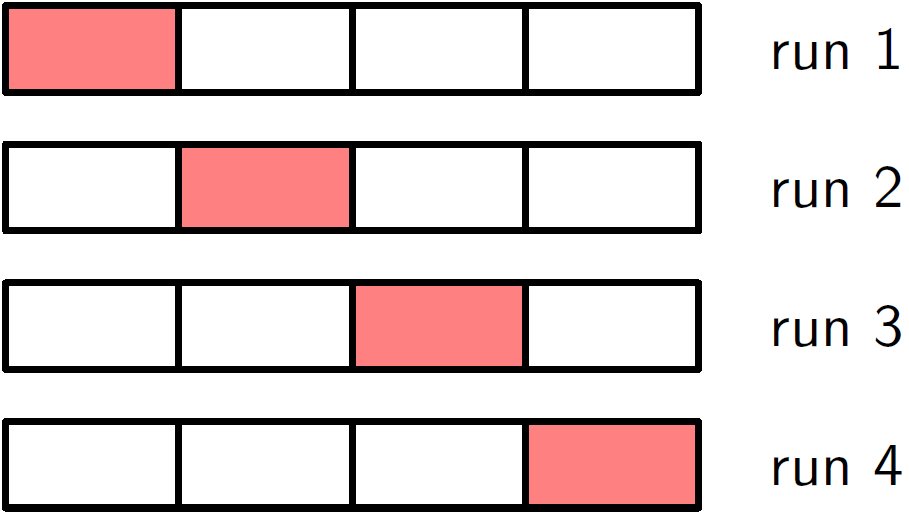
\includegraphics[width=0.5\linewidth ]{figures/crossv.png}
    \centering
    \caption{Cross validation for S=4 \cite{bishop2006pattern}.}
    \label{fig:crossv}
\end{figure}



\textcolor{red}{add about neural networks}\\